\subsubsection{IMDb Dataset}

The IMDb dataset is a well-known dataset in the machine learning community. It contains 50,000 reviews from IMDb and has a limit of 30 reviews per movie\cite{maas-EtAl:2011:ACL-HLT2011}. It is noteworthy that the dataset is balanced in terms of positive and negative reviews, which are equally represented. When creating the dataset, reviews with a score of 4 out of 10 were considered negative and those with a score of 7 out of 10 were considered positive. Neural reviews were excluded to maintain the quality of the dataset. The dataset is divided into training and testing datasets, each with an equal portion. To ensure fairness and accuracy in the results, the dataset creators have taken special care to keep the training and testing datasets balanced.

% \begin{figure}[H]
%     \centering
%     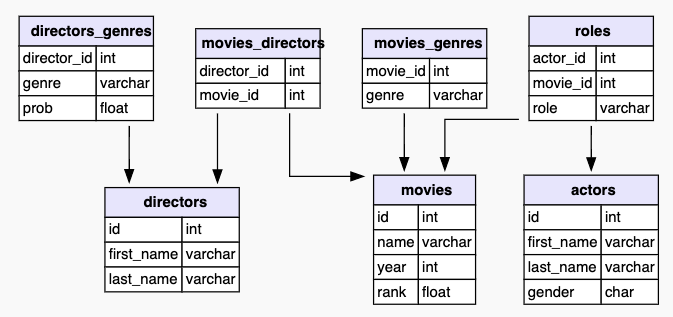
\includegraphics[width=0.8\textwidth]{pics/db/IMDb.png}
%     \caption{Database Structure of IMDb dataset\cite{dahl-etal-1994-expanding}}
%     \label{fig:IMDb}
% \end{figure}

\begin{figure}[H]
    \label{tab:IMDBsqlquery}
    \begin{AIbox}{Example of a complex IMDb SQL query}
        \vspace{-5px}
        \parbox{1\textwidth}{\scriptsize
        \begin{alltt} 
            {\bf Utterance:} \\ 
            What year was the movie The Imitation Game produced?
            \\
            {\bf Query:} \\
            SELECT MOVIEalias0.RELEASE\_YEAR FROM MOVIE AS MOVIEalias0 WHERE MOVIEalias0.TITLE = 'The Imitation Game' ;
        \end{alltt}
        }
        \vspace{-5px}
    \end{AIbox}
\end{figure}

% \begin{table}[H]
%     \centering
%     \caption{Example of a complex IMDb SQL query}
%     \begin{tabular}{|l|p{10cm}|}
%         \hline
%         Utterance & What year was the movie The Imitation Game produced?                                                                       \\ \hline
%         Query  & \small\texttt{SELECT MOVIEalias0.RELEASE\_YEAR FROM MOVIE AS MOVIEalias0 WHERE MOVIEalias0.TITLE = 'The Imitation Game' ;} \\ \hline
%     \end{tabular}
% \end{table}
